\documentclass[11pt]{article}

\usepackage{amsmath}
\usepackage{mathtools}
\usepackage{amssymb}
\usepackage{wrapfig}
\usepackage{fancyhdr}
\usepackage{tikz-qtree}
\usepackage{tikz-qtree-compat}
\usepackage[normalem]{ulem}
\usepackage{tikz}
\usepackage{graphicx}
\usepackage{lineno}
\usepackage{floatrow}
\usepackage{bm}

\DeclareMathOperator*{\argmin}{argmin}
\DeclareMathOperator*{\argmax}{argmax}

\oddsidemargin0cm
\topmargin-2cm
\textwidth16.5cm
\textheight23.5cm 

\newcommand{\question}[2] {\vspace{.25in} \hrule\vspace{0.5em}
\noindent{\bf #1: #2} \vspace{0.5em}
\hrule \vspace{.10in}}
\renewcommand{\part}[1] {\vspace{.10in} {\bf (#1)}}
\linespread{1.5}

\setlength{\parindent}{0pt}
\setlength{\parskip}{5pt plus 1pt}
 
\DeclarePairedDelimiter\abs{\lvert}{\rvert}%


\begin{document}
\medskip        


\linenumbers


\section{Scaling inference in RNNs with EPI} \label{results_LRRNN}
Transient amplification is a hallmark of neural activity throughout cortex, and is often thought to be intrinsically generated by recurrent connectivity in the responding cortical area \cite{murphy2009balanced, hennequin2014optimal, bondanelli2019population}.
It has been shown that to generate such amplified, yet stabilized responses, the connectivity of RNNs must be non-normal \cite{goldman2009memory, murphy2009balanced}, and satisfy additional constraints \cite{bondanelli2020coding}.
In theoretical neuroscience, RNNs are optimized and then examined to show how dynamical systems could execute a given computation \cite{sussillo2014neural, barak2017recurrent}, but such biologically realistic constraints on connectivity are  ignored during optimization for practical reasons.
In general, access to distributions of connectivity adhering to theoretical criteria like stable amplification, chaotic fluctuations \cite{sompolinsky1988chaos}, or low tangling \cite{russo2018motor} would add great scientific value and contextualization to existing research with RNNs.
Here, we use EPI to learn RNN connectivities producing stable amplification, and demonstrate the superior scalability and efficiency of EPI to alternative approaches.
\begin{figure}
\begin{center}
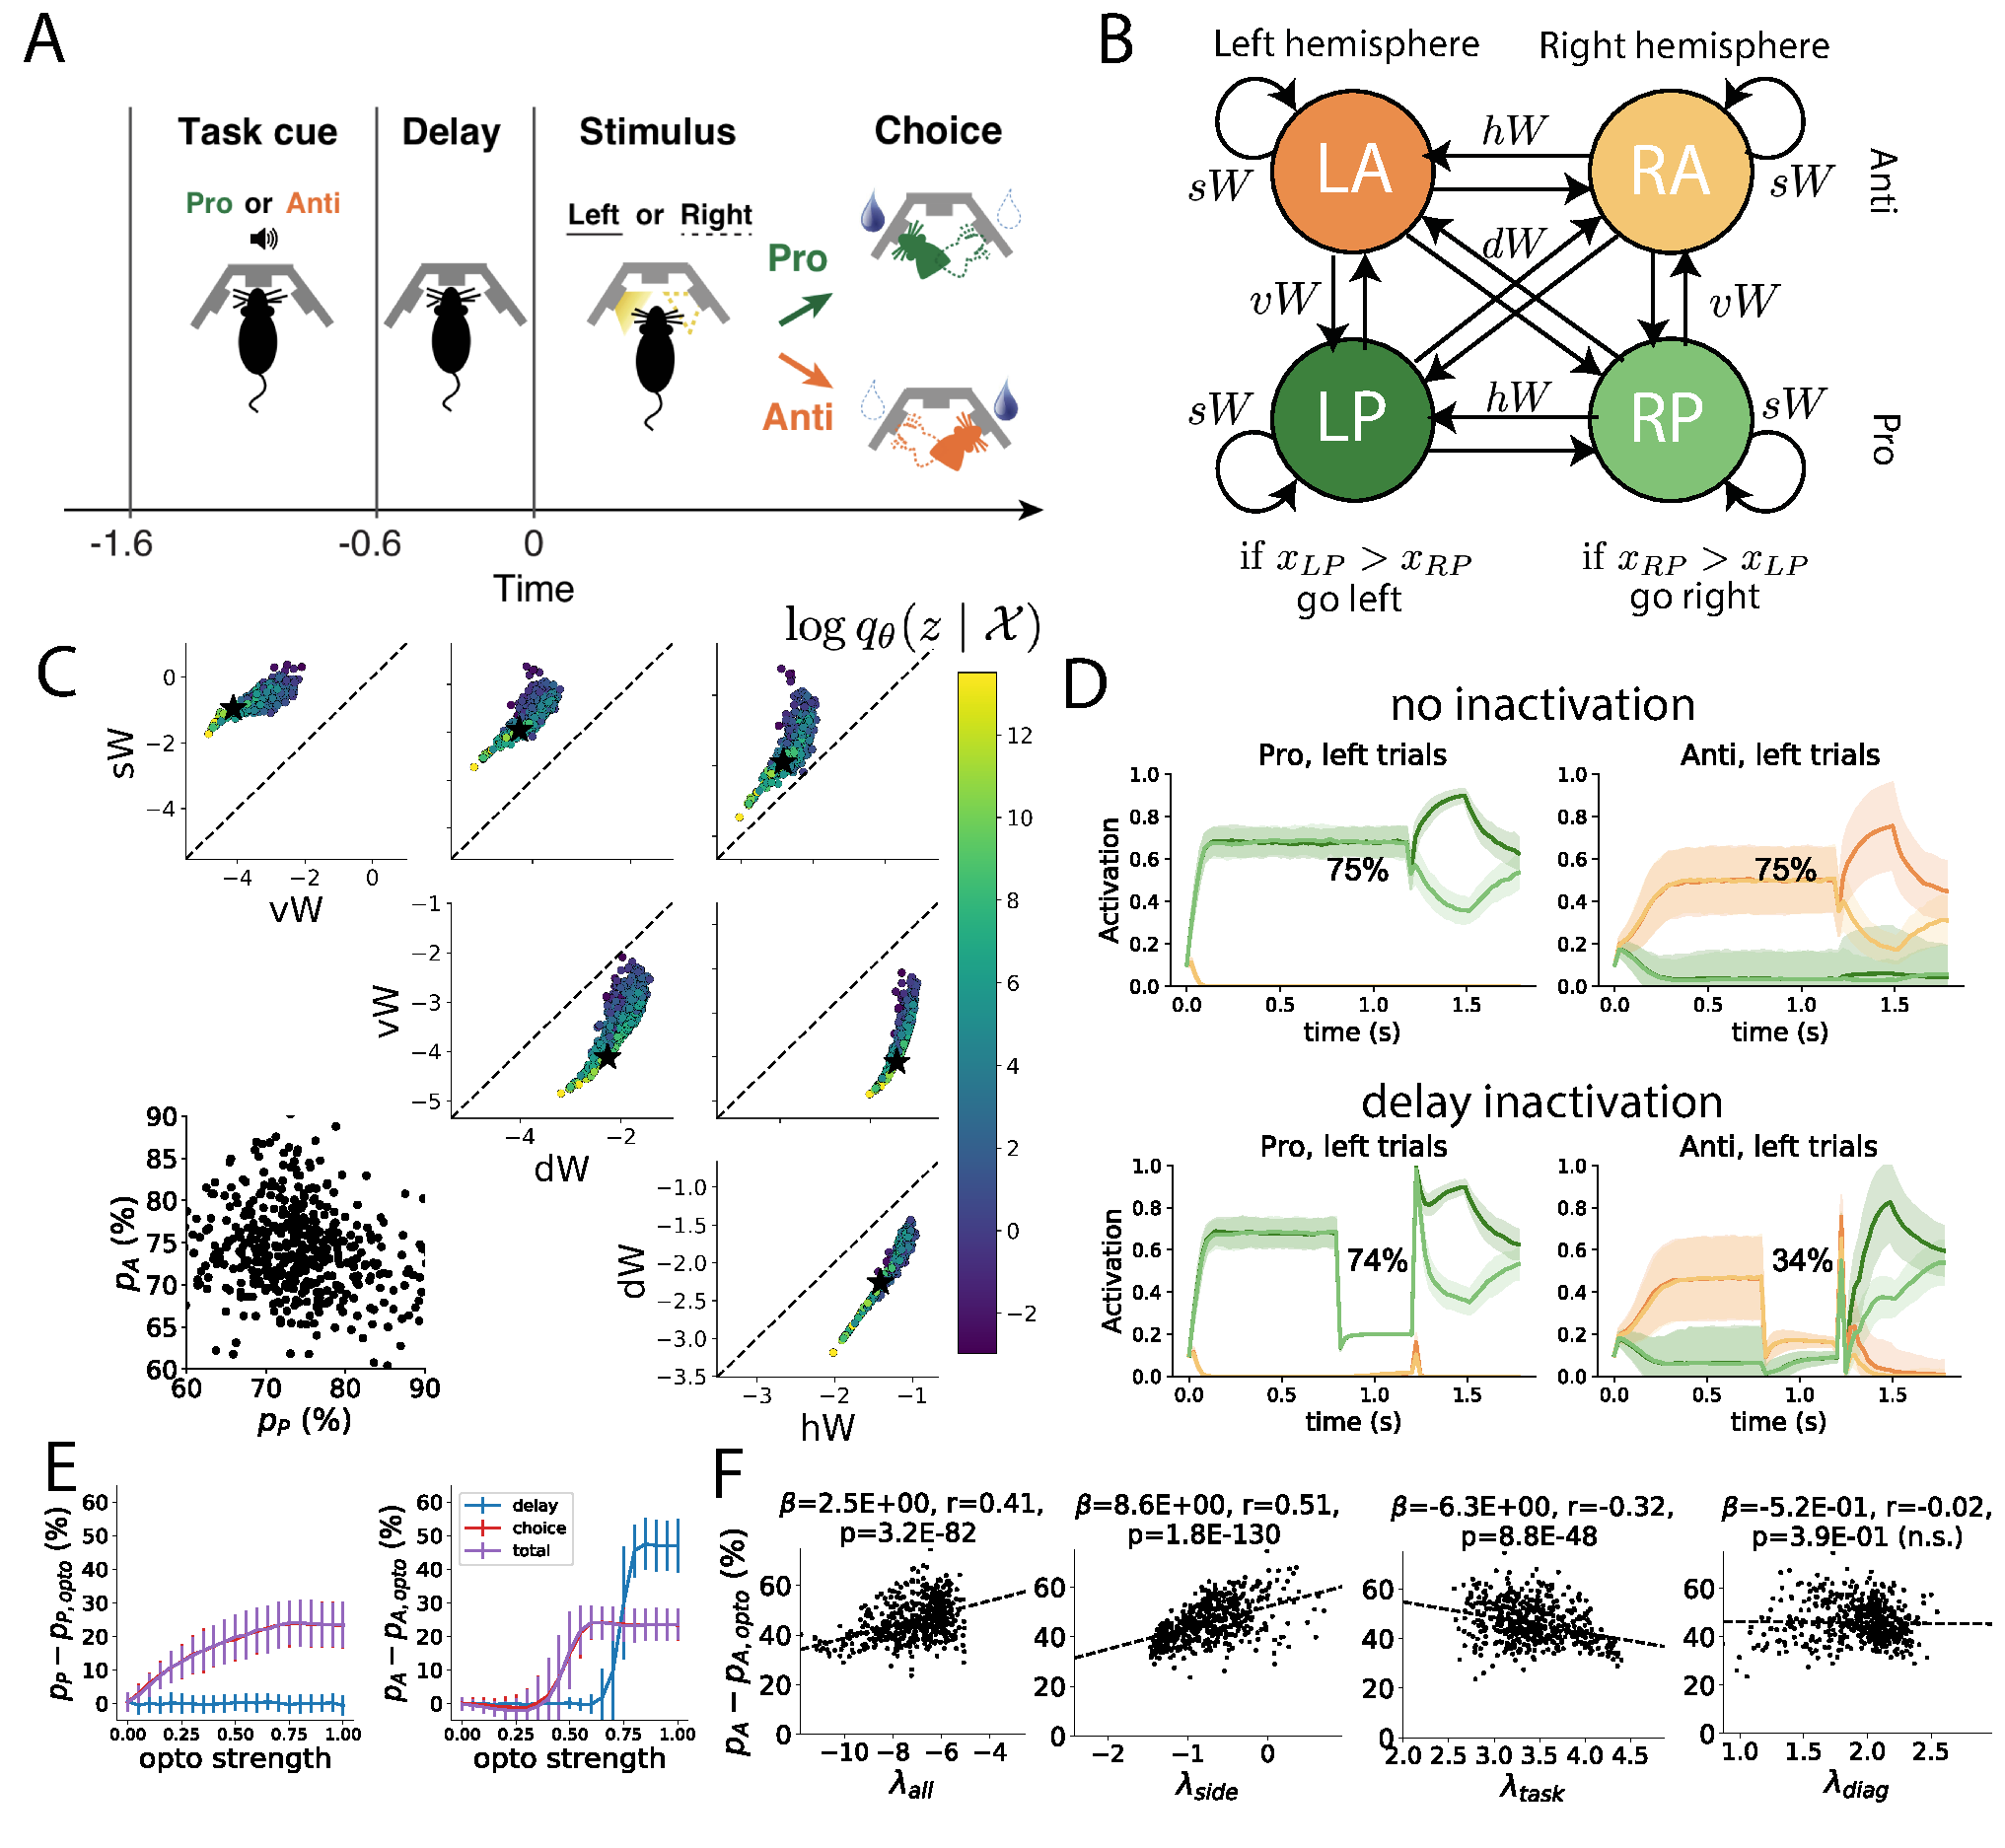
\includegraphics[scale=.8]{figures/fig4/fig4.pdf}
\end{center}
\caption{\small 
\textbf{A}. Wall time of EPI (blue), SNPE (orange), and SMC-ABC (green) to converge on RNN connectivities producing stable amplification.  
Each dot shows convergence time for an individual random seed.
For reference, the mean wall time for EPI to achieve its full constraint convergence (means and variances) is shown (blue line).
\textbf{B}. Simulation count of each algorithm to achieve convergence. Same conventions as A.
\textbf{C}. The predictive distributions of connectivities inferred by EPI (blue), SNPE (orange), and SMC-ABC (green), with reference to $\mathbf{x}_0 = \bm{\mu}$ (gray star).
\textbf{D}. Simulations of networks inferred by each method ($\tau=100ms$).  Each trace (15 per algorithm) corresponds to simulation of one $z$.  (Below) Ratio of obtained samples producing stable amplification, monotonic decay, and instability.
}
\label{fig:LRRNN}
\end{figure}

We consider a rank-2 RNN with N neurons having connectivity $W = UV^\top$
 and dynamics
 \begin{equation}
 \tau \dot{\mathbf{x}} = -\mathbf{x} + W\mathbf{x},
 \end{equation}
where $U = \begin{bmatrix} \mathbf{u}_1 & \mathbf{u}_2 \end{bmatrix} + g \chi^{(W)}$, $V = \begin{bmatrix} \mathbf{v}_1 & \mathbf{v}_2 \end{bmatrix} + g\chi^{(V)}$, $\mathbf{u}_1 \mathbf{u}_2, \mathbf{v}_1, \mathbf{v}_2 \in \left[-1, 1 \right]^N$, and $\chi^{(W)}_{i,j}, \chi^{(V)}_{i,j} \sim \mathcal{N}(0, 1)$.
We infer connectivity parameterizations $\mathbf{z} = \left[\mathbf{u}_1^\top, \mathbf{u}_2^\top, \mathbf{v}_1^\top, \mathbf{v}_2^\top \right]^\top$   that produce stable amplification.
Two conditions are necessary and sufficient for RNNs to exhibit stable amplification \cite{bondanelli2020coding}:  $\text{real}(\lambda_1) < 1$ and
$\lambda^s_1 > 1$, where $\lambda_1$ is the eigenvalue of $W$ with greatest real part and $\lambda^s$ is the maximum eigenvalue of $W^s = \frac{W + W\top}{2}$.
RNNs  with $\text{real}(\lambda_1) = 0.5 \pm 0.5$ and $\lambda_1^s = 1.5 \pm 0.5$ will be stable with modest decay rate ($\text{real}(\lambda_1)$ close to its upper bound of 1) and exhibit modest amplification ($\lambda_1^s$ close to its lower bound of 1).
 EPI can naturally condition on this emergent property
\begin{equation}\label{eq:EP_LRRNN}
\begin{split}
\mathcal{X} ~~:~~ \mathbb{E}_{\mathbf{z}, \mathbf{x}} \begin{bmatrix} \text{real}(\lambda_1) \\ \lambda^s_1 \end{bmatrix} &= \begin{bmatrix} 0.5 \\ 1.5 \end{bmatrix} \\
\text{Var}_{\mathbf{z}, \mathbf{x}} \begin{bmatrix} \text{real}(\lambda_1) \\ \lambda^s_1 \end{bmatrix} &= \begin{bmatrix} 0.25^2 \\ 0.25^2 \end{bmatrix},
\end{split}
\end{equation}
under the notion that variance constraints with standard deviation 0.25 predicate that the vast majority of samples (those within two standard deviations) are within the specified ranges.

For comparison, we infer the parameters $\mathbf{z}$ likely to produce stable amplification using two alternative likelihood-free inference approaches.
We ran sequential Monte Carlo approximate Bayesian computation (SMC-ABC) \cite{sisson2007sequential} and sequential neural posterior estimation (SNPE) \cite{gonccalves2019training} with observation $\mathbf{x}_0 = \bm{\mu}$.
SMC-ABC is a rejection sampling approach that SMC techniques to improve efficiency, and SNPE approximates posteriors with deep probability distributions using a two-network architecture (see Section Related Methods).
Unlike EPI, these statistical inference techniques do not control the mean or variance of the predictive distribution, and these predictions of the inferred posteriors are typically affected by model characteristics (e.g. $N$ and $g$, Fig. \ref{fig:RNN2}).
To compare the efficiency of these different techniques, we measured the time and number of simulations necessary for the distance of the predictive mean to be less than 0.25 from $\bm{\mu} = \mathbf{x}_0$ (see Section \ref{methods_RNN}).

As the number of neurons $N$ in the RNN are scaled, and thus the dimension of the parameter space $\mathbf{z} \in [-1, 1]^{4N}$, we see that EPI converges at greater speed and at greater dimension than SMC-ABC and SNPE (Fig. \ref{fig:LRRNN}A).
It also becomes most efficient to use EPI in terms of simulation count at $N=50$ (Fig. \ref{fig:LRRNN}B).
It is well known that ABC techniques struggle mightily in dimensions greater than about 30 \cite{sisson2018handbook}, yet we were careful to assess the scalability of the more comparable approach SNPE.
Between EPI and SNPE, we closely controlled the number of parameters in deep probability distributions by dimensionality (Fig. \ref{fig:RNN2}), and tested more aggressive SNPE hyperparameterizations when SNPE failed to converge (Fig. \ref{fig:RNN3}).

No matter the number of neurons, EPI always produces connectivity distributions with mean and variance of $\text{real}(\lambda_1)$ and $\lambda_1^s$ according to $\mathcal{X}$ (Fig. \ref{fig:LRRNN}C, blue).
For the dimensionalities in which SMC-ABC is tractable, the inferred parameters are concentrated and offset from $\mathbf{x}_0$ (Fig. \ref{fig:LRRNN}C, green).
When using SNPE the predictions of the inferred parameters are highly concentrated at some RNN sizes and widely varied in others (Fig. \ref{fig:LRRNN}C, orange).
We see these properties reflected in simulations from the inferred distributions: EPI produces a consistent variety of stable, amplified activity norms $|r(t)|$, SMC produces a limited variety of responses, and the changing variety of responses from SNPE emphasizes the control of EPI on parameter predictions.

From this analysis, we see that deep inference techniques EPI and SNPE are far more amenable to inference of high dimensional parameter distributions than rejection sampling techniques like SMC-ABC.
Another benefit over SMC-ABC is that EPI and SNPE offer fast additional samples after optimization.
EPI outperforms SNPE in high dimensions by leveraging gradient information (from $\nabla_\mathbf{z} f(\mathbf{x}; \mathbf{z}) = \nabla_\mathbf{z} [\text{real}(\lambda_1), \lambda_1^s]^\top$) on each optimization iteration.
Through this example, we've shown that EPI can be used for insight into RNNs with respect to their theoretical properties, and that when $\nabla_\mathbf{z} f(\mathbf{x}; \mathbf{z})$ is tractable, EPI can be used to efficiently infer high dimensional parameter distributions in mechanistic models of neural computation.

\bibliography{eLife2020}
\bibliographystyle{unsrt}

\subsection{Methods}\label{methods_RNN}
We examine the scaling properties of EPI by learning connectivities of RNNs of increasing size that exhibit stable amplification.
Rank-2 RNN connectivity is modeled as $W = UV^\top$, where $U = \begin{bmatrix} \mathbf{u}_1 & \mathbf{u}_2 \end{bmatrix} + g \chi^{(W)}$, $V = \begin{bmatrix} \mathbf{v}_1 & \mathbf{v}_2 \end{bmatrix} + g\chi^{(V)}$, and $\chi^{(W)}_{i,j}, \chi^{(V)}_{i,j} \sim \mathcal{N}(0, 1)$.
This RNN model has dynamics
\begin{equation}
\tau \dot{\mathbf{x}} = -\mathbf{x} + W\mathbf{x}.
\end{equation}
In this analysis, we infer connectivity parameterizations $\mathbf{z} = \left[\mathbf{u}_1^\top, \mathbf{u}_2^\top, \mathbf{v}_1^\top, \mathbf{v}_2^\top \right]^\top \in \left[-1, 1 \right]^{(4N)}$   that produce stable amplification using EPI, SMC-ABC \cite{sisson2007sequential}, and SNPE \cite{gonccalves2019training} (see Section Related Methods).

For this RNN model to be stable, all real eigenvalues of $W$ must be less than 1:  $\text{real}(\lambda_1) < 1$, where $\lambda_1$ denotes the greatest real eigenvalue of $W$.
For a stable RNN to amplify at least one input pattern, the symmetric connectivity $W^s = \frac{W + W\top}{2}$ must have an eigenvalue greater than 1:
$\lambda^s_1 > 1$, where  $\lambda^s$ is the maximum eigenvalue of $W^s$.
These two conditions are necessary and sufficient for stable amplification in RNNs \cite{bondanelli2020coding}.
We define the emergent property of stable amplification with means of these eigenvalues (0.5 and 1.5, respectively) that satisfy these conditions.
To complete the emergent property definition, we chose variances ($0.25^2$) about those means such that samples rarely violate the eigenvalue constraints.
In terms of the EPI optimization variables, this is written as
\begin{equation} 
T(\mathbf{x}; \mathbf{z}) = \begin{bmatrix} \text{real}(\lambda_1)(\mathbf{x}; \mathbf{z}) \\ \lambda_1^s(\mathbf{x}; \mathbf{z}) \\ \left(\text{real}(\lambda_1)(\mathbf{x}; \mathbf{z}) - 0.5 \right)^2 \\ \left( \lambda_1^s(\mathbf{x}; \mathbf{z})  - 1.5 \right)^2 \end{bmatrix},
\end{equation}
\begin{equation} 
\bm{\mu}_{\text{opt}} = \begin{bmatrix} 0.5 \\ 1.5 \\ 0.25^2 \\ 0.25^2 \end{bmatrix}.
\end{equation}
Gradients of maximum eigenvalues of Hermitian matrices like $W^s$ are available with modern automatic differentiation tools.
To differentiate through the $\text{real}(\lambda_1)$, we solve the following equation for eigenvalues of rank-2 matrices using the rank reduced matrix $W^r = V^{\top} U$
\begin{equation}
\lambda_{\pm} = \frac{\text{Tr}(W^r) \pm \sqrt{\text{Tr}(W^r)^2 - 4\text{Det}(W^r)}}{2}.
\end{equation}

For EPI in Fig. \ref{fig:LRRNN}, we used a real NVP architecture with three coupling layers of affine transformations parameterized by two-layer neural networks of 100 units per layer.
The initial distribution was a standard isotropic gaussian $z_0 \sim \mathcal{N}(\mathbf{0}, I)$ mapped to the support of $\mathbf{z}_i \in [-1, 1]$. 
We used an augmented Lagrangian coefficient of $c_0 = 10^{3}$, a batch size $n=200$, $\beta=4$, and chose to use $500$ iterations per augmented Lagrangian epoch and emergent property constraint convergence was evaluated at $N_{\text{test}} = 200$ (Fig. \ref{fig:LRRNN}B blue line, and Fig. \ref{fig:LRRNN}C-D blue).

We compared EPI to two alternative likelihood-free inference (LFI) techniques, since the likelihood of these eigenvalues given $\mathbf{z}$ is not available.
Approximate Bayesian computation (ABC) \cite{beaumont2002approximate} is a rejection sampling technique for obtaining sets of parameters $\mathbf{z}$ that produce activity $\mathbf{x}$ close to some observed data $\mathbf{x}_0$.
Sequential Monte Carlo approximate Bayesian computation (SMC-ABC) is the state-of-the-art ABC method, which leverages SMC techniques to improve sampling speed.
We ran SMC-ABC with the pyABC package \cite{klinger2018pyabc} to infer RNNs with stable amplification: connectivities having eigenvalues within an $\epsilon$-defined $l$-$2$ distance of
\begin{equation}\label{eq:stab_amp_x0}
x_0 = \begin{bmatrix} \text{real}(\lambda_1) \\ \lambda^s_1 \end{bmatrix} = \begin{bmatrix} 0.5 \\ 1.5 \end{bmatrix}.
\end{equation}
SMC-ABC was run with a uniform prior over $\mathbf{z} \in \left[-1, 1 \right]^{(4N)}$, a population size of 1,000 particles with simulations parallelized over 32 cores, and a multivariate normal transition model.

\begin{figure}
\begin{center}
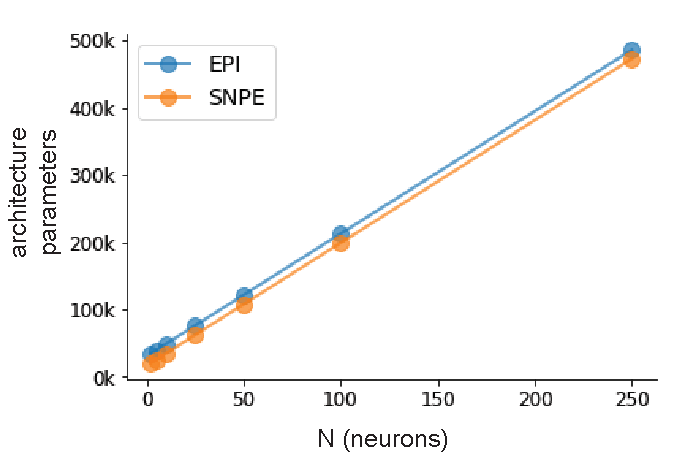
\includegraphics[scale=0.7]{figures/figRNN2/figRNN2.pdf}
\end{center}
\caption{\small (RNN1): 
Number of parameters in deep probability distribution architectures of EPI (blue) and SNPE (orange) by RNN size ($N$).
}
\label{fig:RNN1}
\end{figure}

SNPE, the next LFI approach in our comparison, is far more similar to EPI.
Like EPI, SNPE models parameters in mechanistic models with deep probability distributions, yet their learning algorithms are categorically different.
SNPE uses a two-network architecture to approximate the posterior distribution of the model conditioned on observed data $\mathbf{x}_0$.
The amortizing network maps observations $\mathbf{x}_i$ to the parameters of the deep probability distribution. 
The weights and biases of the parameter network are optimized by sequentially augmenting the training data with additional pairs ($\mathbf{z}_i$, $\mathbf{x}_i$) based on the most recent posterior approximation.
This sequential procedure is important to get training data $\mathbf{z}_i$ to be closer to the true posterior, and $\mathbf{x}_i$ to be closer to the observed data.
For the deep probability distribution architecture, we chose a masked autoregressive flow with affine couplings (the default choice), three transforms, 50 hidden units, and a normalizing flow mapping to the support as in EPI.
This architectural choice closely tracked the size of the architecture used by EPI (Fig. \ref{fig:RNN1}).
As in SMC-ABC, we ran SNPE with $\mathbf{x}_0 = \mu$.
All SNPE optimizations were run for a limit of 1.5 days on a Tesla V100 GPU, or until two consecutive rounds resulted in a validation log probability lower than the maximum observed.

\begin{figure}
\begin{center}
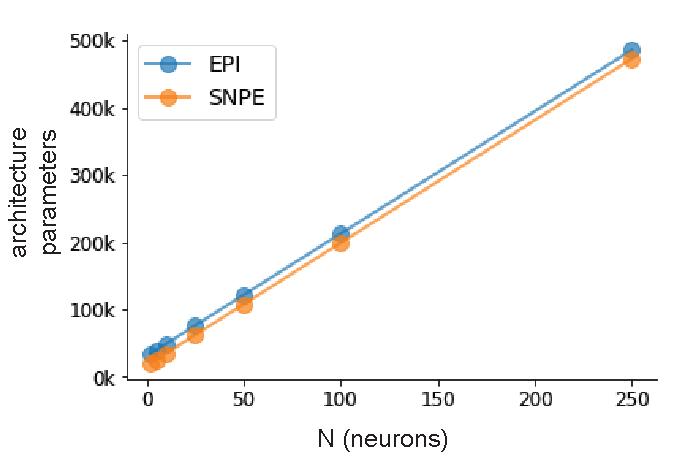
\includegraphics[scale=0.8]{figures/figRNN1/figRNN1.pdf}
\end{center}
\caption{\small (RNN2): Model characteristics affect predictions of posteriors inferred by SNPE, while predictions of parameters inferred by EPI remain fixed.
\textbf{A}. Predictive distribution of EPI (blue) and SNPE (orange) inferred connectivity of RNNs exhibiting stable amplification with $N=2$ (top), $N=10$ (bottom), $g=0.01$ (left), and $g=0.1$ (right).
\textbf{B}. Entropy of parameter distribution approximations throughout optimization with $N=2$ (top), $N=10$ (bottom), $g=0.1$ (dark shade), and $g=0.01$ (light shade).
\textbf{C}. Validation log probabilities throughout SNPE optimization. Same conventions as B.
\textbf{D}. Adherence to EPI constraints. Same conventions as B.
}
\label{fig:RNN2}
\end{figure}

To clarify the difference in objectives of EPI and SNPE, we show their results on RNN models with different numbers of neurons $N$ and random strength $g$.  
The parameters inferred by EPI consistently produces the same mean and variance of $\text{real}(\lambda_1)$ and $\lambda_1^s$, while those inferred by SNPE change according to the model definition (Fig. \ref{fig:RNN2}A).
For $N=2$ and $g=0.01$, the SNPE posterior has greater concentration in eigenvalues around $\mathbf{x}_0$ than at $g=0.1$, where the model has greater uncertainty (Fig. \ref{fig:RNN2}B top, orange).
At both levels of $g$ when $N=2$, the posterior of SNPE has lower entropy than EPI at convergence (Fig. \ref{fig:RNN2}B top).
However at $N=10$, SNPE results in a predictive distribution of more widely dispersed eigenvalues (Fig. \ref{fig:RNN2}A bottom), and an inferred posterior with greater entropy than EPI (Fig. \ref{fig:RNN2}B bottom).
We highlight these differences not to focus on an insightful trend, but to emphasize that these methods optimize different objectives with different implications.

Note that SNPE converges when it's validation log probability has saturated after several rounds of optimization (Fig. \ref{fig:RNN2}C), and that EPI converges after several epochs of its own optimization to enforce the emergent property constraints (Fig. \ref{fig:RNN2}D blue).
Importantly, as SNPE optimizes its posterior approximation, the predictive means change, and at convergence may be different than $\mathbf{x}_0$ (Fig. \ref{fig:RNN2}D orange, left).
It is sensible to assume that predictions of a well-approximated SNPE posterior should closely reflect the data on average (especially given a uniform prior and a low degree of stochasticity), however this is not a given.
Furthermore, no aspect of the SNPE optimization controls the variance of the predictions (Fig. \ref{fig:RNN2}D orange, right).

To compare the efficiency of these algorithms for inferring RNN connectivity distributions producing stable amplification, we develop a convergence criteria that can be used across methods.
While EPI has its own hypothesis testing convergence criteria for the emergent property, it would not make sense to use this criteria on SNPE and SMC-ABC which do not constrain the means and variances of their predictions.
Instead, we consider EPI and SNPE to have converged after completing its most recent optimization epoch (EPI) or round (SNPE) in which the distance
\begin{equation}
d(q_\theta(z)) = |\mathbb{E}_{\mathbf{z}, \mathbf{x}} \left[f(\mathbf{x}; \mathbf{z}) \right] - \bm{\mu}|_2
\end{equation}
is less than 0.25.
We consider SMC-ABC to have converged once the population produces samples within the $\epsilon = 0.5$ ball ensuring stable amplification.

\begin{figure}
\begin{center}
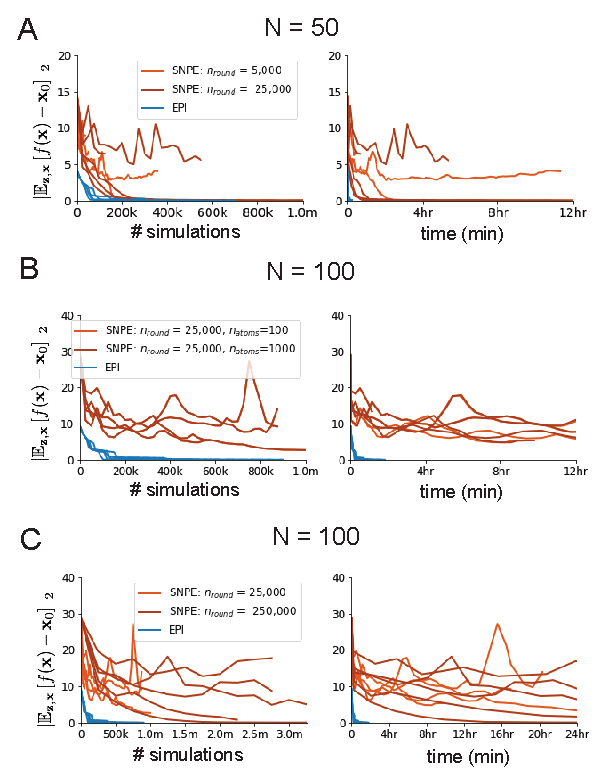
\includegraphics[scale=1.]{figures/figRNN3/figRNN3.pdf}
\end{center}
\caption{\small (RNN3): 
SNPE convergence was enabled by increasing $n_{\text{round}}$, not $n_{\text{atom}}$.
\textbf{A}. Difference of mean predictions $\mathbf{x}_0$ throughout optimization at $N=50$ with by simulation count (left) and wall time (right) of SNPE with $n_{\text{round}} = 5,000$ (light orange), SNPE with $n_{\text{round}} = 25,000$ (dark orange), and EPI (blue).
Each line shows an individual random seed.
\textbf{B}. Same conventions as A at $N=100$ of SNPE with $n_{\text{atom}} = 100$ (light orange) and $n_{\text{atom}} = 1,000$ (dark orange).
\textbf{C}. Same conventions as A at $N=100$ of SNPE with $n_{\text{round}} = 25,000$ (light orange) and $n_{\text{round}} = 250,000$ (dark orange).
}
\label{fig:RNN3}
\end{figure}

When assessing the scalability of SNPE, it is important to check that alternative hyperparamterizations could not yield better performance.
Key hyperparameters of the SNPE optimization are the number of simulations per round $n_{\text{round}}$, the number of atoms used in the atomic proposals of the SNPE-C algorithm \cite{greenberg2019automatic}, and the batch size $n$.
To match EPI, we used a batch size of $n = 200$ for $N <= 25$, however we found $n=1,000$ to be helpful for SNPE in higher dimensions.
While $n_{\text{round}} = 1,000$ yielded SNPE convergence for $N <= 25$, we found that a substantial increase to $n_{\text{round}} = 25,000$ yielded more consistent convergence at $N=50$ (Fig. \ref{fig:RNN3}A).
By increasing $n_{\text{round}}$, we also necessarily increase the duration of each round.
At $N=100$, we tried two hyperparameter modifications.
As suggested in \cite{greenberg2019automatic}, we increased $n_{\text{atom}}$ by an order of magnitude to improve gradient quality, but this had little effect on the optimization (much overlap between same random seeds) (Fig. \ref{fig:RNN3}B).
Finally, we increased $n_{\text{round}}$ by an order of magnitude, which yielded convergence in one case, but no others.
We found no way to improve the convergence rate of SNPE without making more aggressive hyperparameter choices requiring high numbers of simulations.

In Figure \ref{fig:LRRNN}C-D, we show samples form the random seed resulting in emergent property convergence at greatest entropy (EPI), the random seed resulting in greatest validation log probability (SNPE), and the result of all converged random seeds (SMC).


\end{document}

